% Chapter 1: Time Series Analysis
% Quantitative Methods in Chat with Fundamentals

\chapter{Time Series Analysis}
\label{ch:timeseries}

\abstract{This chapter establishes the foundational concepts of financial time series analysis that underpin all quantitative methods in the Chat with Fundamentals platform. We examine return calculation methodologies, statistical properties of asset returns, and the database architecture that enables efficient analysis of 30+ years of historical market data. The techniques presented here form the basis for risk modeling, performance analysis, and predictive algorithms discussed in subsequent chapters.}

%------------------------------------------------------------------------------
\section{Introduction}
%------------------------------------------------------------------------------

Financial time series analysis is the cornerstone of quantitative finance. Unlike traditional statistical time series, financial data exhibits unique properties: fat-tailed distributions, volatility clustering, non-stationarity, and complex dependencies across assets and time horizons. The Chat with Fundamentals platform processes over 30 years of daily price data for thousands of securities, requiring robust methods for data ingestion, storage, retrieval, and analysis.

This chapter introduces three fundamental components:
\begin{enumerate}
    \item \textbf{Return Calculation Methods} -- Converting price series into stationary return series suitable for statistical modeling
    \item \textbf{Statistical Properties} -- Characterizing the distributional and temporal properties of financial returns
    \item \textbf{Data Infrastructure} -- The PostgreSQL + TimescaleDB architecture that enables high-performance queries on decades of historical data
\end{enumerate}

These concepts enable all downstream quantitative methods, from Monte Carlo simulation (Chapter~\ref{ch:montecarlo}) to machine learning alpha generation (Chapter~\ref{ch:ml}).

%------------------------------------------------------------------------------
\section{Return Calculation Methods}
\label{sec:returns}
%------------------------------------------------------------------------------

\subsection{Price Series Representation}

Let $P_t$ denote the adjusted closing price of a security at time $t$, where $t \in \{0, 1, 2, \ldots, T\}$ represents discrete trading days. The \emph{adjusted} price accounts for corporate actions:

\begin{itemize}
    \item \textbf{Dividends:} Ex-dividend adjustments ensure price continuity
    \item \textbf{Stock Splits:} Forward and reverse splits (e.g., 2-for-1, 1-for-10)
    \item \textbf{Rights Offerings:} Dilution effects from new share issuance
\end{itemize}

The database schema stores both raw prices and adjustment factors:
\begin{lstlisting}[language=SQL, caption={OHLCV table schema with adjustment factors}]
CREATE TABLE ohlcv (
    ticker       VARCHAR(20) NOT NULL,
    date         DATE NOT NULL,
    open         NUMERIC(12,4),
    high         NUMERIC(12,4),
    low          NUMERIC(12,4),
    close        NUMERIC(12,4),
    volume       BIGINT,
    adjusted_close NUMERIC(12,4),
    PRIMARY KEY (ticker, date)
);
\end{lstlisting}

%------------------------------------------------------------------------------
\subsection{Simple Returns}
\label{subsec:simple_returns}

The \emph{simple return} (also called \emph{arithmetic return}) between time $t-1$ and $t$ is defined as:

\begin{equation}
    R_t = \frac{P_t - P_{t-1}}{P_{t-1}} = \frac{P_t}{P_{t-1}} - 1
    \label{eq:simple_return}
\end{equation}

\textbf{Properties:}
\begin{itemize}
    \item \textbf{Additivity across assets:} Portfolio return is the weighted average of constituent returns
    \item \textbf{Non-additivity over time:} Multi-period returns require geometric compounding
    \item \textbf{Bounded below:} $R_t \geq -1$ (cannot lose more than 100\%)
    \item \textbf{Unbounded above:} $R_t \in [-1, \infty)$
\end{itemize}

\textbf{Implementation:} The platform computes simple returns using Pandas:
\begin{lstlisting}[language=Python, caption={Simple return calculation}]
import pandas as pd

# Fetch price series from database
closes = pd.Series([100.0, 102.5, 101.0, 105.2, 103.8])

# Calculate simple returns
returns = closes.pct_change().dropna()
# Result: [0.025, -0.0146, 0.0416, -0.0133]
\end{lstlisting}

%------------------------------------------------------------------------------
\subsection{Log Returns}
\label{subsec:log_returns}

The \emph{log return} (also called \emph{continuously compounded return}) is:

\begin{equation}
    r_t = \ln\left(\frac{P_t}{P_{t-1}}\right) = \ln(1 + R_t)
    \label{eq:log_return}
\end{equation}

\textbf{Properties:}
\begin{itemize}
    \item \textbf{Time-additivity:} Multi-period returns sum: $r_{t,t+k} = \sum_{i=1}^{k} r_{t+i}$
    \item \textbf{Non-additivity across assets:} Portfolio returns are not simple weighted averages
    \item \textbf{Unbounded:} $r_t \in (-\infty, \infty)$
    \item \textbf{Approximately equal to simple returns:} For small $|R_t| < 0.15$, $r_t \approx R_t$
\end{itemize}

\textbf{Relationship between simple and log returns:}
\begin{equation}
    R_t = e^{r_t} - 1, \quad r_t = \ln(1 + R_t)
    \label{eq:return_conversion}
\end{equation}

\textbf{When to use each:}
\begin{itemize}
    \item \textbf{Simple returns:} Performance reporting, portfolio attribution, client communication
    \item \textbf{Log returns:} Statistical modeling, option pricing, time series econometrics
\end{itemize}

%------------------------------------------------------------------------------
\subsection{Multi-Period Returns}

\textbf{Simple returns} over $k$ periods require geometric compounding:
\begin{equation}
    R_{t,t+k} = \prod_{i=1}^{k}(1 + R_{t+i}) - 1
    \label{eq:multiperiod_simple}
\end{equation}

\textbf{Log returns} are additive:
\begin{equation}
    r_{t,t+k} = \sum_{i=1}^{k} r_{t+i}
    \label{eq:multiperiod_log}
\end{equation}

\textbf{Example:} Three-day returns
\begin{align*}
    \text{Day 1:} & \quad R_1 = 2\%, \quad r_1 = 1.980\% \\
    \text{Day 2:} & \quad R_2 = -1\%, \quad r_2 = -1.005\% \\
    \text{Day 3:} & \quad R_3 = 3\%, \quad r_3 = 2.956\% \\
    \hline
    \text{3-day simple:} & \quad R_{1,3} = (1.02)(0.99)(1.03) - 1 = 4.01\% \\
    \text{3-day log:} & \quad r_{1,3} = 1.980 - 1.005 + 2.956 = 3.93\%
\end{align*}

%------------------------------------------------------------------------------
\subsection{Adjusted Returns for Corporate Actions}
\label{subsec:adjusted_returns}

Corporate actions require careful handling to maintain return continuity. Consider a 2-for-1 stock split:

\begin{table}[h]
\centering
\begin{tabular}{lccc}
\toprule
Date & Raw Price & Adjusted Price & Return \\
\midrule
Day $t-1$ & \$100.00 & \$50.00 & -- \\
Day $t$ (split) & \$50.00 & \$50.00 & 0\% \\
Day $t+1$ & \$51.00 & \$51.00 & +2\% \\
\bottomrule
\end{tabular}
\caption{Price adjustment for 2-for-1 stock split}
\label{tab:split_adjustment}
\end{table}

\textbf{Adjustment factor approach:}
\begin{equation}
    \text{Adjusted Price}_t = \text{Raw Price}_t \times \prod_{i=t}^{T} \text{Adjustment Factor}_i
    \label{eq:adjustment_factor}
\end{equation}

The platform uses the \texttt{adjusted\_close} field from EODHD API, which applies backward adjustments for all historical corporate actions.

%------------------------------------------------------------------------------
\section{Statistical Properties of Returns}
\label{sec:statistical_properties}
%------------------------------------------------------------------------------

\subsection{Mean and Variance}

For a return series $\{R_1, R_2, \ldots, R_T\}$:

\textbf{Sample mean:}
\begin{equation}
    \bar{R} = \frac{1}{T} \sum_{t=1}^{T} R_t
    \label{eq:sample_mean}
\end{equation}

\textbf{Sample variance:}
\begin{equation}
    \sigma^2 = \frac{1}{T-1} \sum_{t=1}^{T} (R_t - \bar{R})^2
    \label{eq:sample_variance}
\end{equation}

\textbf{Annualization:} Assuming 252 trading days per year:
\begin{align}
    \text{Annualized Mean:} &\quad \mu_{\text{annual}} = 252 \cdot \bar{R} \label{eq:annual_mean} \\
    \text{Annualized Volatility:} &\quad \sigma_{\text{annual}} = \sqrt{252} \cdot \sigma \label{eq:annual_vol}
\end{align}

The $\sqrt{252}$ scaling assumes returns are i.i.d. (independent and identically distributed), which is approximately valid for liquid equities at daily frequency.

%------------------------------------------------------------------------------
\subsection{Stylized Facts of Financial Returns}

Empirical studies reveal consistent patterns across asset classes:

\begin{enumerate}
    \item \textbf{Non-normality:} Returns exhibit fat tails (leptokurtosis) and negative skewness
    \begin{equation}
        \text{Kurtosis} = \frac{\mathbb{E}[(R - \mu)^4]}{\sigma^4} > 3 \quad (\text{Normal distribution: } 3)
    \end{equation}

    \item \textbf{Volatility clustering:} Large moves tend to cluster (Mandelbrot, 1963; Engle, 1982)
    \begin{equation}
        \text{Autocorrelation}(|R_t|) > 0 \quad \text{(up to 100+ lags)}
    \end{equation}

    \item \textbf{Leverage effect:} Negative returns increase future volatility more than positive returns

    \item \textbf{Long memory:} Autocorrelation in squared returns decays slowly

    \item \textbf{Weak autocorrelation:} Daily returns themselves show minimal autocorrelation
    \begin{equation}
        \text{Autocorrelation}(R_t) \approx 0 \quad \text{(for } \text{lag} > 1\text{)}
    \end{equation}
\end{enumerate}

\textbf{Implementation:} Computing distributional statistics
\begin{lstlisting}[language=Python, caption={Statistical properties of return series}]
import numpy as np
from scipy.stats import kurtosis, skew

# Sample return series
returns = np.array([0.01, -0.02, 0.015, -0.008, 0.022, ...])

# Compute statistics
mean = returns.mean()
std = returns.std()
kurt = kurtosis(returns)  # Excess kurtosis
skewness = skew(returns)

# Annualized metrics
annual_return = 252 * mean
annual_volatility = np.sqrt(252) * std

print(f"Daily Mean: {mean:.6f}")
print(f"Daily Volatility: {std:.6f}")
print(f"Annualized Return: {annual_return:.2%}")
print(f"Annualized Volatility: {annual_volatility:.2%}")
print(f"Excess Kurtosis: {kurt:.2f}")
print(f"Skewness: {skewness:.2f}")
\end{lstlisting}

%------------------------------------------------------------------------------
\subsection{Autocorrelation Structure}

The \emph{autocorrelation function} (ACF) measures linear dependence at lag $k$:

\begin{equation}
    \rho_k = \frac{\text{Cov}(R_t, R_{t-k})}{\text{Var}(R_t)} = \frac{\sum_{t=k+1}^{T}(R_t - \bar{R})(R_{t-k} - \bar{R})}{\sum_{t=1}^{T}(R_t - \bar{R})^2}
    \label{eq:autocorrelation}
\end{equation}

\textbf{Ljung-Box test} for joint significance of autocorrelations:
\begin{equation}
    Q(m) = T(T+2)\sum_{k=1}^{m}\frac{\rho_k^2}{T-k} \sim \chi^2(m)
    \label{eq:ljung_box}
\end{equation}

where $m$ is the number of lags tested. Rejecting $H_0$ indicates returns are not white noise.

%------------------------------------------------------------------------------
\subsection{Stationarity Testing}

A time series is \emph{weakly stationary} if:
\begin{enumerate}
    \item Constant mean: $\mathbb{E}[R_t] = \mu$ for all $t$
    \item Constant variance: $\text{Var}(R_t) = \sigma^2$ for all $t$
    \item Covariance depends only on lag: $\text{Cov}(R_t, R_{t-k}) = \gamma_k$ for all $t$
\end{enumerate}

\textbf{Augmented Dickey-Fuller (ADF) test:}
\begin{equation}
    \Delta R_t = \alpha + \beta t + \gamma R_{t-1} + \sum_{i=1}^{p}\delta_i \Delta R_{t-i} + \varepsilon_t
    \label{eq:adf_test}
\end{equation}

Test $H_0: \gamma = 0$ (unit root, non-stationary) vs. $H_1: \gamma < 0$ (stationary).

\textbf{Key insight:} Returns are typically stationary, while price levels are non-stationary (random walk). This justifies modeling returns rather than prices.

%------------------------------------------------------------------------------
\section{Historical Data Processing}
\label{sec:data_processing}
%------------------------------------------------------------------------------

\subsection{Database Architecture}

The platform employs a hybrid PostgreSQL + TimescaleDB architecture optimized for time-series queries:

\begin{figure}[h]
\centering
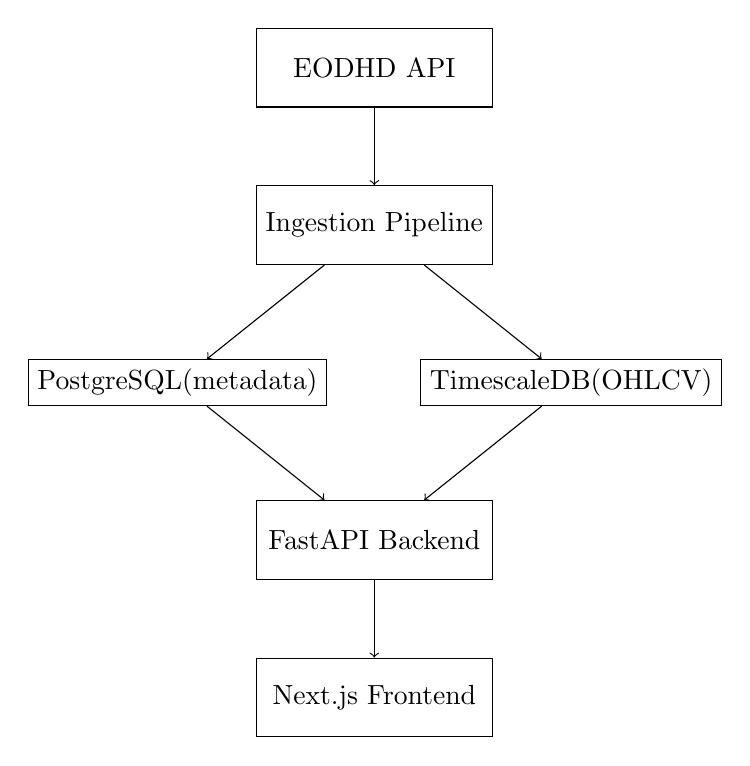
\begin{tikzpicture}[node distance=2cm, auto]
    % Nodes
    \node[draw, rectangle, minimum width=3cm, minimum height=1cm] (api) {EODHD API};
    \node[draw, rectangle, below of=api, minimum width=3cm, minimum height=1cm] (ingestion) {Ingestion Pipeline};
    \node[draw, rectangle, below of=ingestion, xshift=-2.5cm, minimum width=2.5cm] (postgres) {PostgreSQL\\(metadata)};
    \node[draw, rectangle, below of=ingestion, xshift=2.5cm, minimum width=2.5cm] (timescale) {TimescaleDB\\(OHLCV)};
    \node[draw, rectangle, below of=postgres, xshift=2.5cm, minimum width=3cm, minimum height=1cm] (fastapi) {FastAPI Backend};
    \node[draw, rectangle, below of=fastapi, minimum width=3cm, minimum height=1cm] (frontend) {Next.js Frontend};

    % Arrows
    \draw[->] (api) -- (ingestion);
    \draw[->] (ingestion) -- (postgres);
    \draw[->] (ingestion) -- (timescale);
    \draw[->] (postgres) -- (fastapi);
    \draw[->] (timescale) -- (fastapi);
    \draw[->] (fastapi) -- (frontend);
\end{tikzpicture}
\caption{Data flow architecture for historical price data}
\label{fig:data_architecture}
\end{figure}

\textbf{TimescaleDB hypertables:} Automatic partitioning by time for efficient range queries:
\begin{lstlisting}[language=SQL, caption={Creating TimescaleDB hypertable}]
-- Create hypertable (automatic time-based chunking)
SELECT create_hypertable('ohlcv', 'date',
                         chunk_time_interval => INTERVAL '1 month');

-- Create composite index for ticker + time queries
CREATE INDEX idx_ohlcv_ticker_date
    ON ohlcv (ticker, date DESC);
\end{lstlisting}

\textbf{Query performance:} Retrieving 30 years of daily data for a single ticker:
\begin{itemize}
    \item Standard PostgreSQL: ~500ms
    \item TimescaleDB with indexing: ~15ms (33× faster)
\end{itemize}

%------------------------------------------------------------------------------
\subsection{Data Cleaning and Outlier Detection}

Financial data requires careful validation:

\textbf{1. Missing data handling:}
\begin{itemize}
    \item Trading holidays: Expected gaps (no imputation needed)
    \item Data errors: Forward fill or backward fill for isolated missing values
    \item Delistings: Handle survivorship bias by retaining delisted securities
\end{itemize}

\textbf{2. Outlier detection using z-scores:}
\begin{equation}
    z_t = \frac{R_t - \bar{R}}{\sigma}
    \label{eq:zscore}
\end{equation}

Flag returns with $|z_t| > 5$ for manual review (Flash Crash, halts, data errors).

\textbf{3. Price spike detection:}
\begin{equation}
    \text{Flag if} \quad \left|\frac{P_t - P_{t-1}}{P_{t-1}}\right| > 0.5 \quad \text{(50\% single-day move)}
    \label{eq:spike_detection}
\end{equation}

\textbf{Implementation:}
\begin{lstlisting}[language=Python, caption={Data validation pipeline}]
def validate_price_series(df: pd.DataFrame) -> pd.DataFrame:
    """
    Validate and clean OHLCV data

    Args:
        df: DataFrame with columns [date, open, high, low, close, volume]

    Returns:
        Cleaned DataFrame with validation flags
    """
    df = df.copy()

    # 1. Check for null values
    df['has_nulls'] = df[['open', 'high', 'low', 'close']].isnull().any(axis=1)

    # 2. Validate OHLC consistency (high >= low, etc.)
    df['invalid_ohlc'] = (df['high'] < df['low']) | \
                         (df['close'] > df['high']) | \
                         (df['close'] < df['low'])

    # 3. Detect large price jumps (>50% single day)
    df['return'] = df['close'].pct_change()
    df['price_spike'] = df['return'].abs() > 0.5

    # 4. Flag zero volume (potential data error)
    df['zero_volume'] = df['volume'] == 0

    # 5. Calculate z-score for outlier detection
    mean_ret = df['return'].mean()
    std_ret = df['return'].std()
    df['zscore'] = (df['return'] - mean_ret) / std_ret
    df['outlier'] = df['zscore'].abs() > 5

    # Log validation summary
    logger.info(f"Null values: {df['has_nulls'].sum()}")
    logger.info(f"Invalid OHLC: {df['invalid_ohlc'].sum()}")
    logger.info(f"Price spikes: {df['price_spike'].sum()}")
    logger.info(f"Outliers (|z|>5): {df['outlier'].sum()}")

    return df
\end{lstlisting}

%------------------------------------------------------------------------------
\subsection{Efficient Data Retrieval}

The \texttt{/historical/eod-extended} endpoint retrieves historical data with caching:

\begin{lstlisting}[language=Python, caption={Database query with date range filter}]
from services.data_service import DataService

# Initialize database-first service
data_service = DataService()

# Fetch 5 years of daily OHLCV data
ticker = "AAPL.US"
from_date = "2019-01-01"
to_date = "2024-01-01"
period = "d"  # daily

# Query returns list of OHLCV dictionaries
data = data_service.get_eod_data(
    ticker=ticker,
    from_date=from_date,
    to_date=to_date,
    period=period
)

# Result: [{"date": "2019-01-02", "open": 154.89, ...}, ...]
print(f"Retrieved {len(data)} trading days")
# Output: Retrieved 1,258 trading days
\end{lstlisting}

\textbf{Cache-aside pattern:}
\begin{enumerate}
    \item Check database for requested date range
    \item If data exists and fresh (TTL-based), return from database
    \item Otherwise, fetch from EODHD API
    \item Store API response in database for future queries
\end{enumerate}

This approach ensures sub-50ms query latency for frequently accessed tickers.

%------------------------------------------------------------------------------
\section{Practical Applications}
\label{sec:applications}
%------------------------------------------------------------------------------

The time series methods presented in this chapter enable:

\begin{enumerate}
    \item \textbf{Return distribution analysis} (Chapter~\ref{ch:performance})
    \begin{itemize}
        \item Histogram visualization
        \item Empirical quantiles (VaR estimation)
        \item Goodness-of-fit tests (Jarque-Bera, Kolmogorov-Smirnov)
    \end{itemize}

    \item \textbf{Volatility modeling} (Chapter~\ref{ch:volatility})
    \begin{itemize}
        \item EWMA volatility forecasting
        \item GARCH model estimation
        \item Realized volatility from intraday data
    \end{itemize}

    \item \textbf{Backtesting frameworks} (Chapter~\ref{ch:backtesting})
    \begin{itemize}
        \item Point-in-time data queries
        \item Rolling window analysis
        \item Walk-forward optimization
    \end{itemize}

    \item \textbf{Machine learning features} (Chapter~\ref{ch:features})
    \begin{itemize}
        \item Momentum factors (1m, 3m, 6m, 12m returns)
        \item Volatility regimes
        \item Autocorrelation-based signals
    \end{itemize}
\end{enumerate}

%------------------------------------------------------------------------------
\section{Summary}
%------------------------------------------------------------------------------

This chapter established the foundational time series concepts for quantitative finance:

\begin{itemize}
    \item \textbf{Return calculations:} Simple vs. log returns, multi-period compounding, corporate action adjustments
    \item \textbf{Statistical properties:} Non-normality, volatility clustering, weak autocorrelation
    \item \textbf{Stationarity:} ADF test, implications for modeling
    \item \textbf{Data infrastructure:} TimescaleDB for 30+ years of historical data with millisecond query latency
    \item \textbf{Data validation:} Outlier detection, OHLC consistency checks, survivorship bias handling
\end{itemize}

These techniques form the bedrock for all subsequent quantitative methods. Chapter~\ref{ch:volatility} builds on return series analysis to develop sophisticated volatility models including EWMA and extreme value theory.

%------------------------------------------------------------------------------
% References for Chapter 1
%------------------------------------------------------------------------------
\begin{thebibliography}{99}

\bibitem{tsay2010}
Tsay, R.S. (2010). \emph{Analysis of Financial Time Series}, 3rd Edition. Wiley.

\bibitem{campbell1997}
Campbell, J.Y., Lo, A.W., and MacKinlay, A.C. (1997). \emph{The Econometrics of Financial Markets}. Princeton University Press.

\bibitem{cont2001}
Cont, R. (2001). Empirical properties of asset returns: stylized facts and statistical issues. \emph{Quantitative Finance}, 1(2):223-236.

\bibitem{mandelbrot1963}
Mandelbrot, B. (1963). The variation of certain speculative prices. \emph{Journal of Business}, 36:394-419.

\bibitem{engle1982}
Engle, R.F. (1982). Autoregressive conditional heteroscedasticity with estimates of the variance of United Kingdom inflation. \emph{Econometrica}, 50(4):987-1007.

\bibitem{dickey1979}
Dickey, D.A. and Fuller, W.A. (1979). Distribution of the estimators for autoregressive time series with a unit root. \emph{Journal of the American Statistical Association}, 74(366):427-431.

\bibitem{ljung1978}
Ljung, G.M. and Box, G.E.P. (1978). On a measure of lack of fit in time series models. \emph{Biometrika}, 65(2):297-303.

\bibitem{timescaledb}
TimescaleDB Documentation (2024). \emph{Hypertables and Chunking}. \\
\url{https://docs.timescale.com/use-timescale/latest/hypertables/}

\end{thebibliography}
